
%\documentclass[tikz,convert={convertexe={magick.exe}}]{standalone}
\documentclass[tikz,convert]{standalone}
\usetikzlibrary{arrows}

\usepackage{ifthen}

\begin{document}
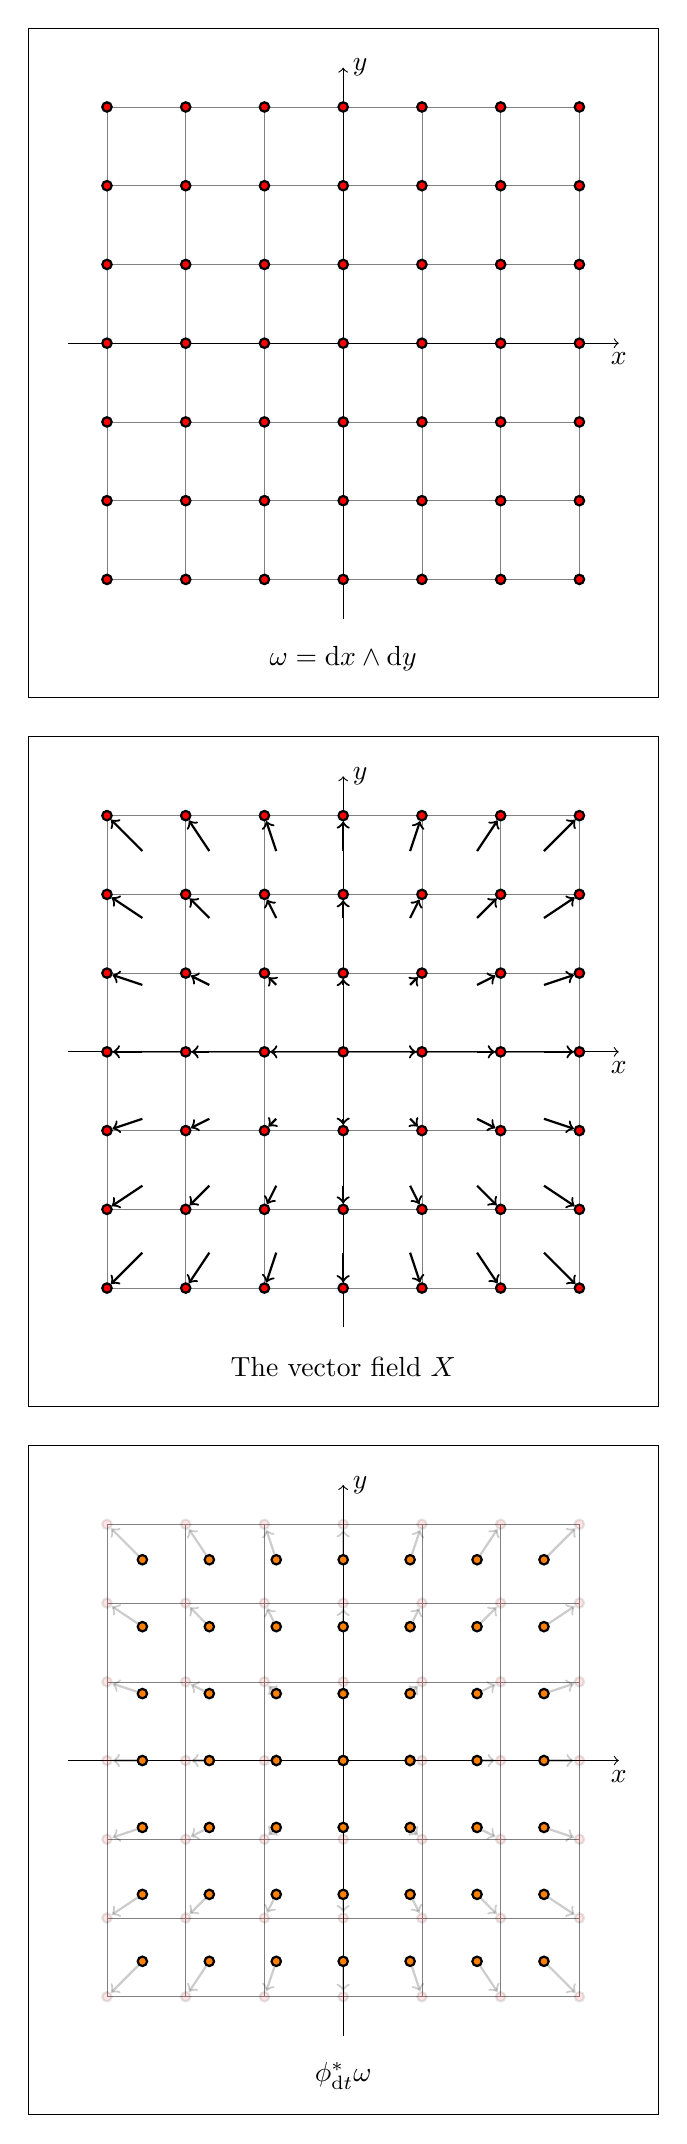
\begin{tikzpicture}

\tikzstyle atom=[circle, draw, inner sep=1.2pt, fill=red, thick]

\begin{scope}

\foreach \x in {-3,-2,...,3}
\draw[style=help lines, very thin] (\x,-3) -- (\x,3);
\foreach \y in {-3,-2,...,3}
\draw[style=help lines, very thin] (-3,\y) -- (3,\y);

\draw[->] (-3.5,0)--(3.5,0) node[below] {$x$};
\draw[->] (0,-3.5)--(0,3.5) node[right] {$y$};

\foreach \x in {-3,-2,...,3}
\foreach \y in {-3,-2,...,3}
\node[atom] at (\x,\y) {};

\draw (-4,-4.5) rectangle (4,4);
\node at (0,-4) {$\omega = \mathrm{d} x \wedge \mathrm{d} y$};

\end{scope}

\begin{scope}[yshift=-9cm]

\foreach \x in {-3,-2,...,3}
\draw[style=help lines, very thin] (\x,-3) -- (\x,3);
\foreach \y in {-3,-2,...,3}
\draw[style=help lines, very thin] (-3,\y) -- (3,\y);

\draw[->] (-3.5,0)--(3.5,0) node[below] {$x$};
\draw[->] (0,-3.5)--(0,3.5) node[right] {$y$};

\draw (-4,-4.5) rectangle (4,4);
\node at (0,-4) {The vector field $X$};


\foreach \x in {-3,-2,...,3}
\foreach \y in {-3,-2,...,3} {
\node[atom] (\x\y) at (\x,\y) {};
\ifthenelse{\x=0 \and \y=0}{}{
\draw[<-, thick] (\x\y) -- (\x*.85, \y*.85);
}
}
\end{scope}

\begin{scope}[yshift=-18cm]

\foreach \x in {-3,-2,...,3}
\draw[style=help lines, very thin] (\x,-3) -- (\x,3);
\foreach \y in {-3,-2,...,3}
\draw[style=help lines, very thin] (-3,\y) -- (3,\y);

\draw[->] (-3.5,0)--(3.5,0) node[below] {$x$};
\draw[->] (0,-3.5)--(0,3.5) node[right] {$y$};

\draw (-4,-4.5) rectangle (4,4);
\node at (0,-4) {$\phi_{\mathrm{d} t}^* \omega$};

\foreach \x in {-3,-2,...,3}
\foreach \y in {-3,-2,...,3} {
\node[atom, opacity=.1] (A\x\y) at (\x,\y) {};
\node[atom, fill=orange] (B\x\y) at (\x*.85, \y*.85) {};
\ifthenelse{\x=0 \and \y=0}{}{
\draw[<-, thick, opacity=.2] (A\x\y) -- (B\x\y);
}
}
\end{scope}

\end{tikzpicture}
\end{document}